\documentclass[border=6pt]{standalone}
\usepackage{lmodern}
\usepackage[T1]{fontenc}
\usepackage{amsmath}
\usepackage{bm}
\usepackage{xcolor}
\usepackage{tikz}
\usetikzlibrary{arrows.meta,positioning,fit,backgrounds}
\definecolor{cgray}{HTML}{6E6C66}
\definecolor{cblue}{HTML}{2F7DC8}
\definecolor{camber}{HTML}{E0891E}
\definecolor{cgreen}{HTML}{5E9A2E}
\definecolor{cink}{HTML}{2B2B2B}
\newcommand{\dt}[1]{{\scriptsize\textcolor{cink!80}{#1}}}
\tikzset{
  >={Stealth[length=2.2mm]},
  pbox/.style={rounded corners=3pt,draw=cink,line width=0.7pt,align=center,
               text width=2.6cm,minimum height=1.6cm,inner sep=3pt,fill=white},
  num/.style={circle,fill=#1,text=white,font=\bfseries\footnotesize,inner sep=0pt,minimum size=4.6mm},
  note/.style={font=\scriptsize\itshape,text=cink!70,align=center},
  ph/.style={font=\bfseries\footnotesize,text=#1},
}
\begin{document}
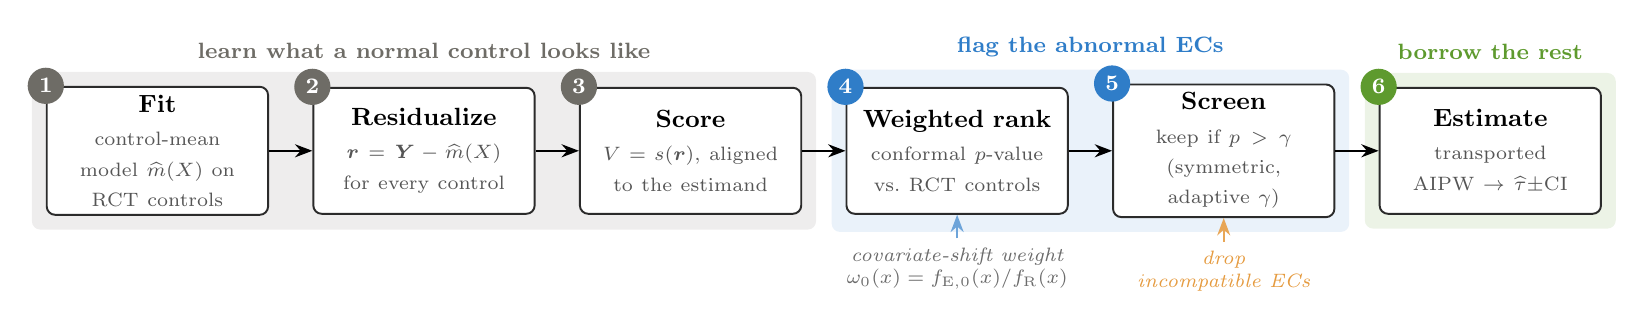
\begin{tikzpicture}[font=\small]

\node[pbox] (s1) {\textbf{Fit}\\[1pt]\dt{control-mean model $\widehat m(X)$ on RCT controls}};
\node[pbox,right=0.55cm of s1] (s2) {\textbf{Residualize}\\[1pt]\dt{$\bm r=\bm Y-\widehat m(X)$ for every control}};
\node[pbox,right=0.55cm of s2] (s3) {\textbf{Score}\\[1pt]\dt{$V=s(\bm r)$, aligned to the estimand}};
\node[pbox,right=0.55cm of s3] (s4) {\textbf{Weighted rank}\\[1pt]\dt{conformal $p$-value vs.\ RCT controls}};
\node[pbox,right=0.55cm of s4] (s5) {\textbf{Screen}\\[1pt]\dt{keep if $p>\gamma$ (symmetric, adaptive $\gamma$)}};
\node[pbox,right=0.55cm of s5] (s6) {\textbf{Estimate}\\[1pt]\dt{transported AIPW $\to\widehat\tau\pm$CI}};

\foreach \a/\b in {s1/s2,s2/s3,s3/s4,s4/s5,s5/s6}
  \draw[->,line width=0.9pt] (\a.east) -- (\b.west);

\foreach \s/\n/\c in {s1/1/cgray,s2/2/cgray,s3/3/cgray,s4/4/cblue,s5/5/cblue,s6/6/cgreen}
  \node[num=\c] at (\s.north west) {\n};

\node[note,below=3mm of s4] (n4) {covariate-shift weight\\ $\omega_0(x)=f_{\mathrm{E},0}(x)/f_{\mathrm R}(x)$};
\draw[->,cblue!70,line width=0.7pt] (n4.north) -- (s4.south);
\node[note,below=3mm of s5,text=camber!85] (n5) {drop\\ incompatible ECs};
\draw[->,camber!75,line width=0.7pt] (n5.north) -- (s5.south);

\begin{scope}[on background layer]
  \node[rounded corners=3pt,fill=cgray!12,fit=(s1)(s3),inner sep=5pt] (pA) {};
  \node[rounded corners=3pt,fill=cblue!10,fit=(s4)(s5),inner sep=5pt] (pB) {};
  \node[rounded corners=3pt,fill=cgreen!12,fit=(s6),inner sep=5pt] (pC) {};
\end{scope}
\node[ph=cgray,above=1pt of pA] {learn what a normal control looks like};
\node[ph=cblue,above=1pt of pB] {flag the abnormal ECs};
\node[ph=cgreen,above=1pt of pC] {borrow the rest};

\end{tikzpicture}
\end{document}
